\chapter{Technical background}\label{chap:theory}

This chapter will address the technical ground necessary to this work.
First comes a quick presentation of FPGAs and how they can be driven from the operating system.

\noindent Follows an overview of Linux operating systems, the distinction between user and kernel mode, and the design of device drivers.

\noindent Next comes an overview of the cryptographic field with the main primitives: message digests, symmetric ciphers and asymmetric ciphers.

\noindent Finally, the ground necessary to understand the inner working and challenges of some VPNs implementations using SSL/TLS and IPsec will be covered.



%%%%%%%%%%%%%%%%%%%%%%%%%%%%%%%%%%%%%%%%%%%%%%%%%%%%%%%%%%%%%%%%%%%%%%%%%%%%%%%%
\section{FPGA}
%%%%%%%%%%%%%%%%%%%%%%%%%%%%%%%%%%%%%%%%%%%%%%%%%%%%%%%%%%%%%%%%%%%%%%%%%%%%%%%%
The aim of this work is to study the impact of offloading cryptographic operations in hardware.
In order to reach that goal, an FPGA will be used.

A Field-Prgrammable Gate Array (FPGA) is an integrated circuit that can be programmed after the manufacturing, using a semiconductor intellectual property core (IP core).
In this work, we will use some of Barco Silex's crypto IP cores.

In order for the operating system to comunicate with the device, they will need to share some memory.
That memory can be directly mapped and accessed from the user-space using \texttt{/dev/mem}, or can use a direct memory access module (DMA).
From the operating system, we build a bunch of scatterlist in the kernel-space memory, then map those pages to memory descriptor that have a physical address on the DMA.
They can be mapped three different ways: \texttt{DMA\_BIDIRECTIONAL}, \texttt{DMA\_TO\_DEVICE} or \texttt{DMA\_FROM\_DEVICE}.
When the CPU write something in those descriptors and synchronize them with the DMA, it does not have to care about them anymore, the DMA in now in charge to send them to the device where registers are ready to read the incomming data.
The same goes from the device to the CPU: when the device wants to communicate data to the OS, it writes it on the DMA that will transfer them to the CPU, triggering a flag on the way to notify it.

\begin{figure}
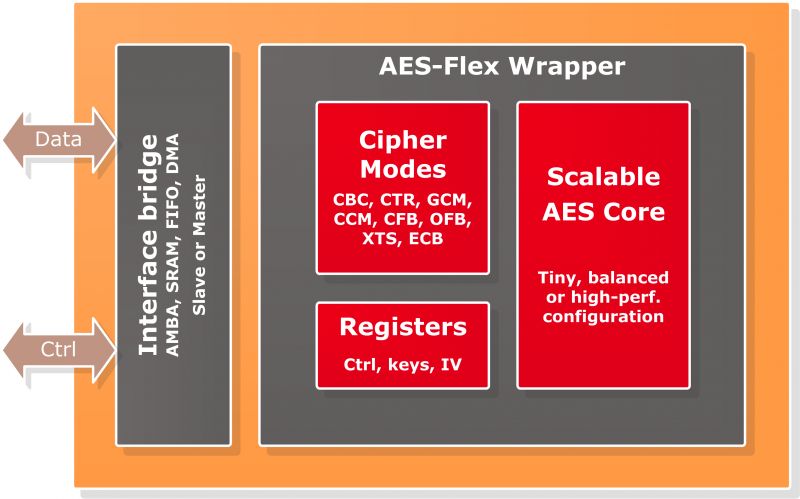
\includegraphics[width=\linewidth]{barco-ba411e-ipcore}
\caption{Barco Silex' AES IP Core}{There are two channels to comunicate with the IP core: the data and control paths~\cite{barco-ba411e}.}
\label{fig:barco-ba411e-ipcore}
\end{figure}

There are two types of interface with such a device: master or slave.
The figure~\ref{fig:barco-ba411e-ipcore}  represent one of Barco Silex' crypto IP cores that proposes two interfaces: one of each type.
\begin{itemize}
	\item The data path is a master. That is the operating system will not have a direct access to the memory registers of the hardware devide. Instead, they will communicate via a DMA bus: one peer places data on the DMA and notifies the other that he can fetch it.
	\item The control (ctrl) path is a slave. The operatin system can directly read and write on this part of the device memory.
\end{itemize}

A master interface has the advantage to offload a part of the memory management to the device, but there is a space overhead to connect the DMA as well as an extra delay to process its data.
A slave interface is usually used for sporadic data, avoiding the overhead of a DMA.
As an example, the data path of Barco Silex' symmetric cryptography IP core is a master, as there is a lot of data to process, whilst the same data path of their asymmetric cryptography IP core is a slave, for the operands are larger and the computation takes more time.



%%%%%%%%%%%%%%%%%%%%%%%%%%%%%%%%%%%%%%%%%%%%%%%%%%%%%%%%%%%%%%%%%%%%%%%%%%%%%%%%
\section{Operating system}
%%%%%%%%%%%%%%%%%%%%%%%%%%%%%%%%%%%%%%%%%%%%%%%%%%%%%%%%%%%%%%%%%%%%%%%%%%%%%%%%

%User/kernel space. Networking application: need to send the data through the kernel: huge overhead.

%Crypto API

\subsection{Device Driver}\label{sec:theory-driver}
% General idea of it works
% device driver in userspace: linux userspace i/o (/dev/mem)
Userspace I/O~\cite{koch2011}

There are two ways to get the status of a hardware device: either by using interruption, or by actively polling the device, relentlessly asking if it finished its operations.
The first case is the cleanest and the most common: when the device has something to send to the driver, or if anything unexpected happened, it sends an interruption request (IRQ) to the processor, which will in turn execute the interruption routine registered by the driver~\citep[chap. 10]{Corbet:2005:LDD:1209083}.
The second case is the easiest and is always guaranteed to work, but won't let go off the processor willingly, loading it at 100\%, and avoiding any other task to be executed.
Fortunately, modern monolithic kernels such as the Linux kernel from 2.6 provide preemptive scheduling~\cite{Santhanam2003}, that is the scheduler interrupts the running task and assigns the processor ressources it used to an other one.
Hence, systems with a lot of processes in need for CPU ressources would not be stalled, but it would not change anything if the only process heavily requesting processor time is the one using the driver.




%%%%%%%%%%%%%%%%%%%%%%%%%%%%%%%%%%%%%%%%%%%%%%%%%%%%%%%%%%%%%%%%%%%%%%%%%%%%%%%%
\section{Cryptography}
%%%%%%%%%%%%%%%%%%%%%%%%%%%%%%%%%%%%%%%%%%%%%%%%%%%%%%%%%%%%%%%%%%%%%%%%%%%%%%%%

Cryptography is the keystone of security. As \citet{Menezes1996} defines it: ``Cryptography is the study of mathematical techniques related to aspects of information security such as confidentiality, data integrity, entity authentication, and data origin authentication."

The four main goals are:
\begin{description}
	\item[Confidentiality] keeping information secret from all but those who are authorized to see it.
	\item[Integrity] ensuring information has not been altered by unauthorized or unknown means.
	\item[Source Authentication] corroborating the source of information.
	\item[Non-repudiation] preventing the denial of previous commitments or actions.
\end{description}

In order to achieve those, four cryptographic primitives are needed: message digests, symmetric and asymmetric ciphers, and digital signatures.








\subsection{Message digest}
%Not the same as digital signature because we use the same key for both MAC values.
A message digest is the result of a one-way mathematical function of a fixed size.
For a given function, each message has a unique digest, comparable to a fingerprint.
Those hash functions are of two types~\cite{infof405}: manipulation detection codes (MDC) to guarantee integrity and message authentication codes (MAC) to guarantee both integrity and source authentication.


An MDC $h(x)$ can follow an iterative construction for a message $x$ including $t$ blocks:
\[
\begin{dcases}
	H_0 = \mbox{initial value}\\
	H_i = f(H_{i-1}, x_i), \mbox{with } i \in [1,t]\\
	h(x) = H_t\\
\end{dcases}
\]

In order to create a MAC, we can add a secret key $k$ to the process, $H_i$ becoming:
\[
	H_i = f(H_{i-1}, x_i, k), \mbox{with } i \in [1,t]\\
\]

HMAC is such function $f()$, as defined in RFC 2104~\cite{rfc2104}
\[
	HMAC(k, x) = h((k\oplus opad)|h((k\oplus ipad)|x))
\]
with a key $k$, and two padding block added for security concerns: an outer pad $opad$ and an inner pad $ipad$.

\noindent There exist a wide varety of MDCs, ranging from block cipher based such as Miyaguchi-Preneel, customized such as MD5, SHA-1 and SHA-2, or built using modular arithmetic such as MASH-1.

In both schemes, data integrity can be guaranteed because the flip of one bit will irremediably change the digest.
However, only a MAC can ensure source authentication since it is the only one based on a shared secret key.

Now rises the question of what and when authenticating.
\citet{Bellare2000} prooved that the most secure solution is to encrypt then compute the MAC from the ciphertext.
We will see in section~\ref{sec:theory-network} that if IPsec follows this recommandation, SSL/TLS does not and MAC first the plaintext then encrypt the message.







\subsection{Symmetric cryptography}
Consider a cryptosystem $(P,C,K,E,D)$, with $P$ and $C$ the spaces of plaintexts and ciphertexts, $E$ and $D$ the encryption and decryption algorithms and a keyspace $K$.
\citet{Menezes1996} and \citet{infof405} define a symmetric scheme as a cryptosystem with two keys $e \in K$ and $d \in K$ respectively associated with the encryption and decryption algorithms.
When using the key pair ($e$, $d$), it should be computationally easy to compute $d$ knowing only $e$, and $e$ from $d$.
In the rest of this work, we will consider the most common case: $e = d$, having thus a single key shared between the peers.

There exists numerous cipher types, and one of the most widespread is the block cipher.
A block cipher splits the message into blocks of fixed size and work on them separately.
An example of such a cipher is illustrated on the figure~\ref{fig:cbc-encrypt} with the Cipher Block Chaining (CBC) mode.
This particular mode is easy to implement and has been robust for a long time, before the rise of the padding oracle attack~\cite{vaudenay2002}.

\indent An other interresting block cipher mode is the Counter (CTR).
Each block of data is treated independently from the others (see figure~\ref{fig:ctr-encrypt}, making the scheme parallelizable and thus more interresting on hardware.

\begin{figure}
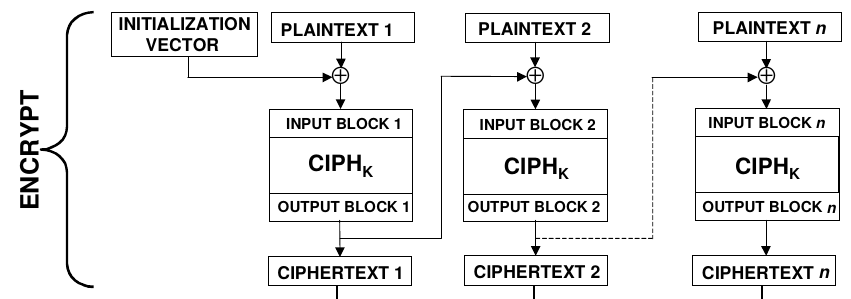
\includegraphics[width=\textwidth]{nist-cbc}
\caption{CBC encryption diagram}{The output of one block is used as the input of the next one. The decryption is very similar. Taken from the NIST recommendation~\cite{nist-sp800-38A}.}
\label{fig:cbc-encrypt}
\end{figure}

\begin{figure}
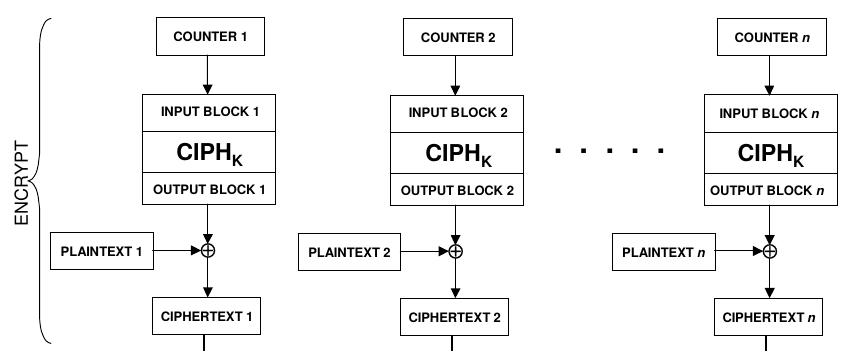
\includegraphics[width=\textwidth]{nist-ctr}
\caption{CTR encryption diagram}{Each block is processed independently from the others. The decryption is very similar. Taken from the NIST recommendation~\cite{nist-sp800-38A}.}
\label{fig:ctr-encrypt}
\end{figure}

Those modes can not work alone and have to be associated with a cipher (``CIPH" on figures~\ref{fig:cbc-encrypt}~and~\ref{fig:ctr-encrypt}).
In 1997, the NIST hosted a competition to choose the successor of the Data Encryption Standard (DES).
In 2000, Rijndael emerged victorious and was renamed Advanced Encryption Standard (AES).
It is still nowadays the most used symmetric block cipher used in a large variety of applications.\newline{}

Most applications want to use confidential and authenticated channels for their sensible communication.
In order to do so, they need to combine a symmetric cipher and a MAC.

\noindent New block cipher have emerged to answer the need for such combinations and formed the Authenticated Encryption with Associated Data (AEAD) mode of operation.
The most widespread mode in network applications is the Galois Counter Mode (GCM, see figure~\ref{fig:gcm-encrypt}), combining the CTR block cipher mode and a GHASH function using multiplications in the Galois field.
The advantage of this mode is that the authentication can be computed in parallel with the encryption, itself parallelizable.
This mode can thus be highly optimized in hardware, as proved Barco Silex with their BA415 IP core reaching up to 100Gbps~\cite{barco-ba415}.

\begin{figure}
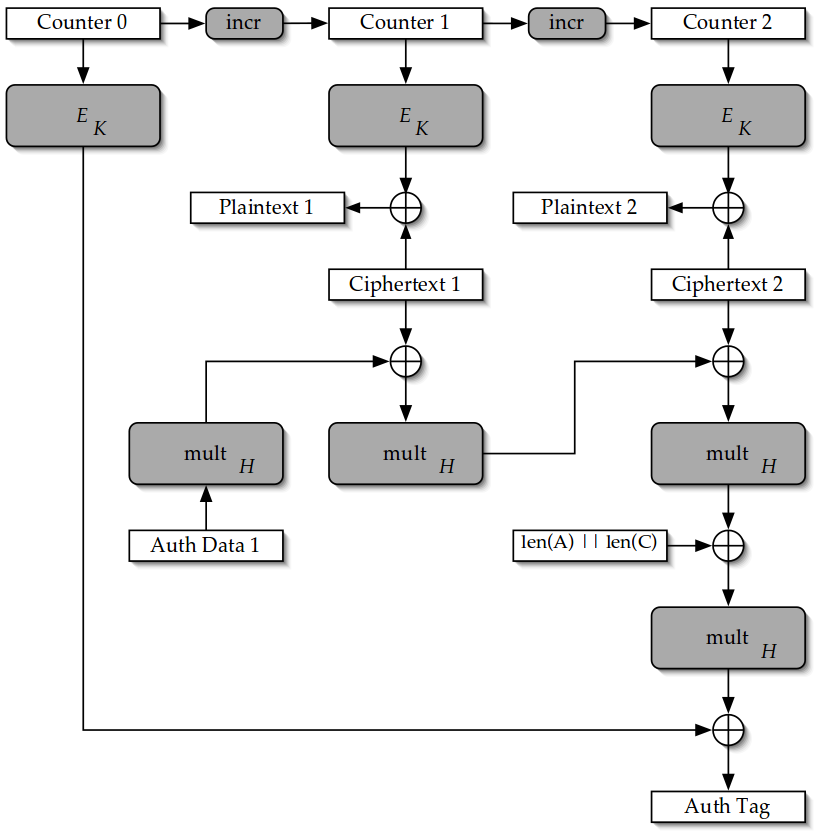
\includegraphics[width=\textwidth]{nist-gcm-encrypt}
\caption{GCM encryption diagram}{taken from the NIST specification~\cite{mcgrew2005}. The ciphertext blocks are formed by \textit{xor}-ing the encrypted counter and the plaintext. The tag is generated by a chain of ciphertext \textit{xor}-ing with Galois field multiplicated data. The decryption works excatly the same way, except the plaintext and ciphertext are swapped.}
\label{fig:gcm-encrypt}
\end{figure}




\subsection{Asymmetric cryptography}
% Diffie-Hellman: show the math about the shared key, maybe from the course INFOH405 or RFC2631, and point which operation will be offloaded.
Asymmetric cryptography relies on a pair of keys: one private known only to the owner of the certificate, and one public available to anyone.
Such cryptography uses two kinds of operations: encryption using the public key of the recipient and digital signature, which is an encryption using the private key of the sender.

\subsubsection{RSA}
RSA is a public-key scheme proposed in 1978 by three MIT researchers (who gave it their name)~\cite{Rivest:1978:MOD:359340.359342}.
A few years later, they founded RSA Laboratories, which is now in charge of maintaining its standards, alongside many others, as the first Public-Key Cryptography Standards, \textit{aka} PKCS \#1.
The last version of the standard is the version 2.2~\cite{pkcs1} and is defined as a precise key generation protocol allowing encryption and decryption.
The keys can be generated by respecting a few steps:
\begin{enumerate}
	\item randomy choose two large primes $p$ and $q$;
	\item compute the modulus $n = p q$, and consequently we have \[\phi(n) = (p-1)(q-1)\]with $\phi(n)$ as the Euler function;
	\item randomly choose the public exponent $e \in ]1,\phi(n)[\ s.t.\ GCD(e,\phi(n)) = 1$;
	\item compute $d \in ]1,\phi(n)[\ s.t.\ e \cdot d \equiv 1 (mod\ \phi(n))$
\end{enumerate}

With those parameters, we can form a public key with the pair $(n, e)$ and a private key with the pair $(n, d)$.

The encryption and decryption of a given message $m \in \mathds{Z}_n$ are defined as follows:
\begin{description}
	\item[Encryption] $c = m^e\ mod\ n$
	\item[Decryption] $m = c^d\ mod\ n$
\end{description}

The scheme is based on modular artihmetic, which is secure because of the factoring problem.
For an opponent to decrypt a ciphertext $c$ wihtout knowing the private key $(d, n)$, he would need to compute the $e^{th}$ roots of $c$, modulo $n$.
This operation is computationally hard, since an efficient solution is yet to be found for sufficiently large key size.


\subsubsection{Diffie-Hellman}
Diffie-Hellman is a secret key exchange protocol: two parties compute a shared secret $ZZ$ that can be used as a symmetric key during the following exchanges.
It uses the same kind of operation as RSA, that is modular exponentiation.
The protocol can be one of three types (\cite{rfc2631}, \cite{Frankel:2005:SGI:2206289}):
\begin{itemize}
	\item Static (DH): the actors use their authenticated certificate to compute the shared secret.
	\item Ephemeral (DHE): the actors create a new pair of public/private keys from which the secret key is derived.
	\item Anonymous: same as ephemeral, but without signing anything, hence not identifying neither of the actors, hence not providing any authentication. This mode is not advisable since it's vulnerable to main-in-the-middle attack.
\end{itemize}
A static scheme is easier to implement and requires much less operations, but using ephemeral keys is essential to ensure perfect forward secrecy.
Imagine that somehow, an opponent lays his hand on the shared secret.
If that secret has already been used, he can decipher all data transfered during past connections.
However, if the secret is new for every new connection, the compromission of the shared secret does not jeopardize past communications.
This is perfect forward secrecy: using a new key to protect the previous messages.

Hereunder is the generation algorithm of an ephemeral shared secret.
For a static secret, Alice and Bob will simply use their static certificate, sparing the modular exponentiation of the ephemeral public key generation.
\begin{enumerate}
	\item Alice generates once $p$ and $g$ (using precomputed parameters):
	\begin{description}[nosep]
		\item[p] large prime number
		\item[g] a generator of $\mathds{Z}_p^*$
	\end{description}
	\item Alice picks a random integer $x_a$ and computes $g^{x_a} mod\ p = y_a$.
	\item Alice sends $p$, $g$ and $y_a$ to Bob, signing everything using her private certificate.
	\item Bob checks the signature and picks $x_b$.
	\item Bob computes $y_a^{x_b} mod\ p = g^{x_a x_b} mod\ p = ZZ$, the shared secret to use as a premaster key from which will be derived the symmetric key for further communications.
	\item Bob sends $y_b = g^{x_b} mod\ p$, signing everything with his private certificate.
	\item Alice checks the signature and computes the same shared secret: $ZZ = y_b^{x_a} mod\ p = g^{x_a x_b} mod\ p$
\end{enumerate}

If the server is Alice, it has to do at least one signature generation, one signature verification and two modular exponentiations.
Note that the client, B in our case, could have one signature less because RFC 5246~\cite{rfc5246} leave it as an optional feature, and the server would then have one verification less.
However, any sane configuration will have both actors signing their ephemeral public key.
If the certificate use RSA, we end up with four modular exponentiations, which can become quite heavy computing wise for certain sizes of key.
We will see in chapter~\ref{chap:results} that while a 1024-bit key size is easily manageable by full software implementation, hardware offloading become a necessity for 4096-bit key sizes.
Moreover, 1024-bit parameter size, both RSA and Diffie-Hellman, are disallowed by the NIST recommandations since 2013~\cite{nist-sp800-131A}.












%%%%%%%%%%%%%%%%%%%%%%%%%%%%%%%%%%%%%%%%%%%%%%%%%%%%%%%%%%%%%%%%%%%%%%%%%%%%%%%%
\section{Network and VPN implementation}\label{sec:theory-network}
%%%%%%%%%%%%%%%%%%%%%%%%%%%%%%%%%%%%%%%%%%%%%%%%%%%%%%%%%%%%%%%%%%%%%%%%%%%%%%%%

% Present the TCP/IP layering
Computer networks are described by two models: the TCP/IP stack and the OSI model, each splitting the network workflow into more or less abstract layers.
The RFC 1122~\cite{rfc1122} defines the TCP/IP, and the international standard ISO/IEC 7498-1~\cite{ISOIEC7498} defines the OSI stack as in the table~\ref{tab:tcp-ip-stack}.
The main difference between the two is the application layer of the TCP/IP stack which corresponds to the three upper layers of the OSI model.
Some references, such as~\citet{tanenbaum2011}, conceptually split the TCP/IP link layer into an additional physical layer.

\begin{table}[ht]
\center
\begin{tabularx}{\textwidth}{|l|l|l|X|} \hline
\multicolumn{2}{|c|}{TCP/IP layering} & \multicolumn{2}{c|}{OSI model} \\ \hline
Layer & Protocols & Layer & Protocols \\ \hline
\multirow{3}{*}{Application} & \multirow{3}{*}{FTP, SSH} & Application & FTP \\ \cline{3-4}
 & & Presentation & ASCII, JPEG \\ \cline{3-4}
 & & Session & RPC, PAP \\ \hline
Transport & TCP, UDP & Transport & TCP, UDP \\ \hline
Internet & IP, ICMP, IPsec & Network & IP, ICMP, IPsec \\ \hline
\multirow{2}{*}{Link} & \multirow{2}{*}{PPP, MAC, Ethernet, L2TP} & Data link & PPP, MAC, Ethernet, L2TP \\ \cline{3-4}
 & & Physical & USB, DSL, IEEE 802.11 \\ \hline
\end{tabularx}
\caption{TCP/IP and OSI model comparison}{They are globaly the same, except for the application layer of the TCP/IP stack which merge togheter the three upper layers of the OSI model. Between parenthsis are examples of protocols resting on each layer.}
\label{tab:tcp-ip-stack}
\end{table}


% First explain what a VPN is.

There exist several major implementations of VPN: SSL, IPsec, L2TP and PPTP.
The later was developped by a vendor consortium leaded by Microsoft and proposed in the RFC 2637 and will not be discussed further.

\noindent L2TP (Layer 2 Tunneling Protocol) is a protocol that simply offers a tunnel without providing confidentiality~\cite{rfc3931}.
A common use case is to combine IPsec and L2TP, as defined in RFC 3193~\cite{rfc3193}.

\subsection{SSL/TLS}
% Introduce SSL/TLS, talk about the protocol, the key exchange and stuff, but leaver OpenVPN for the 'implementation' chapter.
% Question the security? Apparently, it does mac-then-encrypt, which is insecure regarding certain types of attacks \cite{cryptoeprint:2001:045}.
% Plus, SSLv3 is to be deprecated, according to a queued RFC: http://www.rfc-editor.org/internet-drafts/draft-ietf-tls-sslv3-diediedie-03.txt, and is not supported anymore by many servers since poodle.
Application level security.














\subsection{IPsec}
% IPsec as a protocol, strongswan come in the 'implementation' chapter.
IPsec is a protocol whose implementation is a modification of the IP stack in the kernel space.
It is a network/internet level security; it examines incomming IP packets and checks if there exists a security association with the destination, and decrypt it on-the-fly if necessary.

% One of the main disadvantage compared to a user-space VPN is the difficulty to traverse NAT.

IPsec consist of three components~\cite{cryptoencyclopedia2011}, each defined in their respective RFC:
\begin{description}
	\item[Traffic protocols] Encapsulating Security Payload (ESP,~\cite{rfc4303}) and Authentication Header (AH,~\cite{rfc4302}).
	\item[Key management] Internet Key Exchange (IKEv2,~\cite{rfc7296}).
	\item[Policy]Security Policy Database (SPD,~\cite{rfc4301}) and Security Association (SA~\cite{rfc4301}).
\end{description}

As~\citet{Paterson200672} present them, the SAs are used as repository for cryptographic parameters, and the SPD defines the policies to apply.
If the SPD can be populated by hand, typically in a configuration file, the SA management should be left to an automated mechanism: the IKEv2.

\noindent The IKEv2 protocol uses four different types of exchanges to fulfill its role:
\begin{itemize}
	\item \texttt{IKE\_SA\_INIT}: The two peers agree on cryptographic parameters to use. Among these is a Diffie-Hellman shared secret from which are derived symmetric keys used for a special IKE SA.
	\item \texttt{IKE\_AUTH}: Once the peers are protected by the IKE SA, they can authenticate themselves to each other and add a first SA in the SA database (SADB).
	The protocol supports three types of authentication methods:
	\begin{itemize}
		\item Digital signature using a PKI.
		\item MAC using a pre-established secret key.
		\item Extensible Authentication Protocol (EAP) defined in~\citet{rfc3748}.
	\end{itemize}
	At this point, the connection is fully established and ready to use.
	\item \texttt{CREATE\_CHILD\_SA}: Used to create new SAs between the two peers. It may involve new generations of DH secrets to ensure perfect forward secrecy.
	\item \texttt{INFORMATIONAL}: Exchange of management information.
\end{itemize}
~\newline{}

The figure~\ref{fig:esp-packet-structure} shows the structure of an ESP packet.
The ESP header includes two fields: a Security Parameter Index (SPI) and a Sequence Number (SN)
The SPI is a value on which both actors agreed on during the key exchange protocol, identifying the SA to use for the communication.
The SN is an anti-replay feature, an integer incrementing with each packet processed by the SA. This way, the SA will reject any packet that does not have a SN in the current windows, avoiding an intruder to resend a previously captured packet on the network.
As the SN is covered by the integrity, the opponent can not change it without having to change the Integrity Check Value (ICV, \textit{a.k.a.} the message digest).
This authentication covers the whole packet, whilst the confidentiality excludes the ESP header.

\noindent The ESP trailer includes a padding and two 1-byte fields: the padding length and the next header value, which can specify if the packet is dummy or real.
The padding is needed when using block ciphers to obtain a payload which length is an integral multiple of the block length.

\noindent The ESP payload includes an optional IV and an optional Traffic Flow Confidentiality (TFC) padding.
The TFC padding allows to modify the length of the packet with dummy data, somewhat hiding the true nature of the payload.
It differs from the standard padding because its length is not limited to 255 bytes like the latter.

\noindent AH is the same as ESP, except is does not offer encryption features, only the authentication.
Since ESP can use a null cipher, it arguably offers the same features as AH.
The existance of AH is actually historical; when the protocol was developped in the 1990s, there were laws in the United States and other countries preventing the export of product including encryption features.
Having an authentication only counterparty allowed such product to be exported without encryption capabilities.\newline{}

IPsec can be deployed in two modes: 
\begin{itemize}
	\item Transport for end-to-end service and protecting the payload. IPsec examines the incomming payload, checks it has not been tampered with and pass it to the next layer.
	\item Tunnel protects the entire IP packet by encapsulating it into a new IP packet. As the destination contained in the new IP header can be different from the original, this mode can be used to manage gateways.
\end{itemize}
The figure~\ref{fig:ipsec-transport-tunnel} shows the space overhead imposed by AH and ESP in transport and tunnel modes.

Both protocols add 10 bytes of fixed size fields (SPI, SN, pad length and next header).
The other fields are of variable length, or even optional, such as the optional authentication field of minimum 12 bytes, the optional IV of minimum 4 bytes and the padding between 0 and 255 bytes long.
\citet{Xenakis20063225} reached the conclusion in their paper that the use of lightweight -- and deprecated -- encryption schemes (\textit{e.g.} HMAC-MD5 and DES) hardly had any impact on the throughput of the system and on the delay of the packets.
Hence, the space overhead of IPsec is negligible when using more serious schemes (\textit{e.g.} AES-256-CBC with HMAC-SHA-256).


\begin{figure}[ht]
\center
\subfloat[\label{fig:ipsec-transport}Transport]{%
	\large
	\resizebox{.465\linewidth}{!}{%
	% Graphic for TeX using PGF
% Title: /home/para/documents/polytech2015/MA2/Master_thesis/master_thesis/ipsec-transport.dia
% Creator: Dia v0.97.3
% CreationDate: Thu May 21 00:33:06 2015
% For: para
% \usepackage{tikz}
% The following commands are not supported in PSTricks at present
% We define them conditionally, so when they are implemented,
% this pgf file will use them.
\ifx\du\undefined
  \newlength{\du}
\fi
\setlength{\du}{15\unitlength}
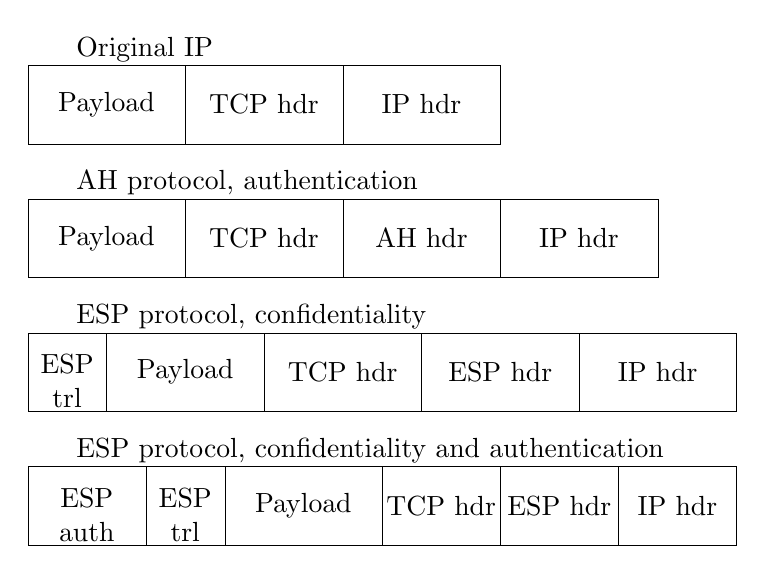
\begin{tikzpicture}
\pgftransformxscale{1.000000}
\pgftransformyscale{-1.000000}
\definecolor{dialinecolor}{rgb}{0.000000, 0.000000, 0.000000}
\pgfsetstrokecolor{dialinecolor}
\definecolor{dialinecolor}{rgb}{1.000000, 1.000000, 1.000000}
\pgfsetfillcolor{dialinecolor}
\pgfsetlinewidth{0.050000\du}
\pgfsetdash{}{0pt}
\pgfsetdash{}{0pt}
\pgfsetmiterjoin
\definecolor{dialinecolor}{rgb}{1.000000, 1.000000, 1.000000}
\pgfsetfillcolor{dialinecolor}
\fill (17.500000\du,15.100000\du)--(17.500000\du,16.100000\du)--(19.000000\du,16.100000\du)--(19.000000\du,15.100000\du)--cycle;
\definecolor{dialinecolor}{rgb}{0.000000, 0.000000, 0.000000}
\pgfsetstrokecolor{dialinecolor}
\draw (17.500000\du,15.100000\du)--(17.500000\du,16.100000\du)--(19.000000\du,16.100000\du)--(19.000000\du,15.100000\du)--cycle;
\pgfsetlinewidth{0.050000\du}
\pgfsetdash{}{0pt}
\pgfsetdash{}{0pt}
\pgfsetmiterjoin
\definecolor{dialinecolor}{rgb}{1.000000, 1.000000, 1.000000}
\pgfsetfillcolor{dialinecolor}
\fill (17.000000\du,13.400000\du)--(17.000000\du,14.400000\du)--(19.000000\du,14.400000\du)--(19.000000\du,13.400000\du)--cycle;
\definecolor{dialinecolor}{rgb}{0.000000, 0.000000, 0.000000}
\pgfsetstrokecolor{dialinecolor}
\draw (17.000000\du,13.400000\du)--(17.000000\du,14.400000\du)--(19.000000\du,14.400000\du)--(19.000000\du,13.400000\du)--cycle;
\pgfsetlinewidth{0.050000\du}
\pgfsetdash{}{0pt}
\pgfsetdash{}{0pt}
\pgfsetmiterjoin
\definecolor{dialinecolor}{rgb}{1.000000, 1.000000, 1.000000}
\pgfsetfillcolor{dialinecolor}
\fill (16.000000\du,11.700000\du)--(16.000000\du,12.700000\du)--(18.000000\du,12.700000\du)--(18.000000\du,11.700000\du)--cycle;
\definecolor{dialinecolor}{rgb}{0.000000, 0.000000, 0.000000}
\pgfsetstrokecolor{dialinecolor}
\draw (16.000000\du,11.700000\du)--(16.000000\du,12.700000\du)--(18.000000\du,12.700000\du)--(18.000000\du,11.700000\du)--cycle;
\pgfsetlinewidth{0.050000\du}
\pgfsetdash{}{0pt}
\pgfsetdash{}{0pt}
\pgfsetmiterjoin
\definecolor{dialinecolor}{rgb}{1.000000, 1.000000, 1.000000}
\pgfsetfillcolor{dialinecolor}
\fill (14.000000\du,10.000000\du)--(14.000000\du,11.000000\du)--(16.000000\du,11.000000\du)--(16.000000\du,10.000000\du)--cycle;
\definecolor{dialinecolor}{rgb}{0.000000, 0.000000, 0.000000}
\pgfsetstrokecolor{dialinecolor}
\draw (14.000000\du,10.000000\du)--(14.000000\du,11.000000\du)--(16.000000\du,11.000000\du)--(16.000000\du,10.000000\du)--cycle;
\pgfsetlinewidth{0.050000\du}
\pgfsetdash{}{0pt}
\pgfsetdash{}{0pt}
\pgfsetmiterjoin
\definecolor{dialinecolor}{rgb}{1.000000, 1.000000, 1.000000}
\pgfsetfillcolor{dialinecolor}
\fill (10.000000\du,10.000000\du)--(10.000000\du,11.000000\du)--(12.000000\du,11.000000\du)--(12.000000\du,10.000000\du)--cycle;
\definecolor{dialinecolor}{rgb}{0.000000, 0.000000, 0.000000}
\pgfsetstrokecolor{dialinecolor}
\draw (10.000000\du,10.000000\du)--(10.000000\du,11.000000\du)--(12.000000\du,11.000000\du)--(12.000000\du,10.000000\du)--cycle;
% setfont left to latex
\definecolor{dialinecolor}{rgb}{0.000000, 0.000000, 0.000000}
\pgfsetstrokecolor{dialinecolor}
\node at (11.000000\du,10.500000\du){Payload};
\pgfsetlinewidth{0.050000\du}
\pgfsetdash{}{0pt}
\pgfsetdash{}{0pt}
\pgfsetmiterjoin
\definecolor{dialinecolor}{rgb}{1.000000, 1.000000, 1.000000}
\pgfsetfillcolor{dialinecolor}
\fill (12.000000\du,10.000000\du)--(12.000000\du,11.000000\du)--(14.000000\du,11.000000\du)--(14.000000\du,10.000000\du)--cycle;
\definecolor{dialinecolor}{rgb}{0.000000, 0.000000, 0.000000}
\pgfsetstrokecolor{dialinecolor}
\draw (12.000000\du,10.000000\du)--(12.000000\du,11.000000\du)--(14.000000\du,11.000000\du)--(14.000000\du,10.000000\du)--cycle;
% setfont left to latex
\definecolor{dialinecolor}{rgb}{0.000000, 0.000000, 0.000000}
\pgfsetstrokecolor{dialinecolor}
\node at (15.000000\du,10.500000\du){IP hdr};
% setfont left to latex
\definecolor{dialinecolor}{rgb}{0.000000, 0.000000, 0.000000}
\pgfsetstrokecolor{dialinecolor}
\node at (13.000000\du,10.500000\du){TCP hdr};
\pgfsetlinewidth{0.050000\du}
\pgfsetdash{}{0pt}
\pgfsetdash{}{0pt}
\pgfsetmiterjoin
\definecolor{dialinecolor}{rgb}{1.000000, 1.000000, 1.000000}
\pgfsetfillcolor{dialinecolor}
\fill (10.000000\du,11.700000\du)--(10.000000\du,12.700000\du)--(12.000000\du,12.700000\du)--(12.000000\du,11.700000\du)--cycle;
\definecolor{dialinecolor}{rgb}{0.000000, 0.000000, 0.000000}
\pgfsetstrokecolor{dialinecolor}
\draw (10.000000\du,11.700000\du)--(10.000000\du,12.700000\du)--(12.000000\du,12.700000\du)--(12.000000\du,11.700000\du)--cycle;
% setfont left to latex
\definecolor{dialinecolor}{rgb}{0.000000, 0.000000, 0.000000}
\pgfsetstrokecolor{dialinecolor}
\node at (11.000000\du,12.200000\du){Payload};
\pgfsetlinewidth{0.050000\du}
\pgfsetdash{}{0pt}
\pgfsetdash{}{0pt}
\pgfsetmiterjoin
\definecolor{dialinecolor}{rgb}{1.000000, 1.000000, 1.000000}
\pgfsetfillcolor{dialinecolor}
\fill (12.000000\du,11.700000\du)--(12.000000\du,12.700000\du)--(14.000000\du,12.700000\du)--(14.000000\du,11.700000\du)--cycle;
\definecolor{dialinecolor}{rgb}{0.000000, 0.000000, 0.000000}
\pgfsetstrokecolor{dialinecolor}
\draw (12.000000\du,11.700000\du)--(12.000000\du,12.700000\du)--(14.000000\du,12.700000\du)--(14.000000\du,11.700000\du)--cycle;
% setfont left to latex
\definecolor{dialinecolor}{rgb}{0.000000, 0.000000, 0.000000}
\pgfsetstrokecolor{dialinecolor}
\node at (17.000000\du,12.200000\du){IP hdr};
% setfont left to latex
\definecolor{dialinecolor}{rgb}{0.000000, 0.000000, 0.000000}
\pgfsetstrokecolor{dialinecolor}
\node at (13.000000\du,12.200000\du){TCP hdr};
\pgfsetlinewidth{0.050000\du}
\pgfsetdash{}{0pt}
\pgfsetdash{}{0pt}
\pgfsetmiterjoin
\definecolor{dialinecolor}{rgb}{1.000000, 1.000000, 1.000000}
\pgfsetfillcolor{dialinecolor}
\fill (14.000000\du,11.700000\du)--(14.000000\du,12.700000\du)--(16.000000\du,12.700000\du)--(16.000000\du,11.700000\du)--cycle;
\definecolor{dialinecolor}{rgb}{0.000000, 0.000000, 0.000000}
\pgfsetstrokecolor{dialinecolor}
\draw (14.000000\du,11.700000\du)--(14.000000\du,12.700000\du)--(16.000000\du,12.700000\du)--(16.000000\du,11.700000\du)--cycle;
% setfont left to latex
\definecolor{dialinecolor}{rgb}{0.000000, 0.000000, 0.000000}
\pgfsetstrokecolor{dialinecolor}
\node at (15.000000\du,12.200000\du){AH hdr};
% setfont left to latex
\definecolor{dialinecolor}{rgb}{0.000000, 0.000000, 0.000000}
\pgfsetstrokecolor{dialinecolor}
\node[anchor=west] at (10.500000\du,9.800000\du){Original IP};
% setfont left to latex
\definecolor{dialinecolor}{rgb}{0.000000, 0.000000, 0.000000}
\pgfsetstrokecolor{dialinecolor}
\node[anchor=west] at (10.500000\du,11.500000\du){AH protocol, authentication};
\pgfsetlinewidth{0.050000\du}
\pgfsetdash{}{0pt}
\pgfsetdash{}{0pt}
\pgfsetmiterjoin
\definecolor{dialinecolor}{rgb}{1.000000, 1.000000, 1.000000}
\pgfsetfillcolor{dialinecolor}
\fill (11.000000\du,13.400000\du)--(11.000000\du,14.400000\du)--(13.000000\du,14.400000\du)--(13.000000\du,13.400000\du)--cycle;
\definecolor{dialinecolor}{rgb}{0.000000, 0.000000, 0.000000}
\pgfsetstrokecolor{dialinecolor}
\draw (11.000000\du,13.400000\du)--(11.000000\du,14.400000\du)--(13.000000\du,14.400000\du)--(13.000000\du,13.400000\du)--cycle;
% setfont left to latex
\definecolor{dialinecolor}{rgb}{0.000000, 0.000000, 0.000000}
\pgfsetstrokecolor{dialinecolor}
\node at (12.000000\du,13.900000\du){Payload};
\pgfsetlinewidth{0.050000\du}
\pgfsetdash{}{0pt}
\pgfsetdash{}{0pt}
\pgfsetmiterjoin
\definecolor{dialinecolor}{rgb}{1.000000, 1.000000, 1.000000}
\pgfsetfillcolor{dialinecolor}
\fill (13.000000\du,13.400000\du)--(13.000000\du,14.400000\du)--(15.000000\du,14.400000\du)--(15.000000\du,13.400000\du)--cycle;
\definecolor{dialinecolor}{rgb}{0.000000, 0.000000, 0.000000}
\pgfsetstrokecolor{dialinecolor}
\draw (13.000000\du,13.400000\du)--(13.000000\du,14.400000\du)--(15.000000\du,14.400000\du)--(15.000000\du,13.400000\du)--cycle;
% setfont left to latex
\definecolor{dialinecolor}{rgb}{0.000000, 0.000000, 0.000000}
\pgfsetstrokecolor{dialinecolor}
\node at (18.000000\du,13.900000\du){IP hdr};
% setfont left to latex
\definecolor{dialinecolor}{rgb}{0.000000, 0.000000, 0.000000}
\pgfsetstrokecolor{dialinecolor}
\node at (14.000000\du,13.900000\du){TCP hdr};
\pgfsetlinewidth{0.050000\du}
\pgfsetdash{}{0pt}
\pgfsetdash{}{0pt}
\pgfsetmiterjoin
\definecolor{dialinecolor}{rgb}{1.000000, 1.000000, 1.000000}
\pgfsetfillcolor{dialinecolor}
\fill (15.000000\du,13.400000\du)--(15.000000\du,14.400000\du)--(17.000000\du,14.400000\du)--(17.000000\du,13.400000\du)--cycle;
\definecolor{dialinecolor}{rgb}{0.000000, 0.000000, 0.000000}
\pgfsetstrokecolor{dialinecolor}
\draw (15.000000\du,13.400000\du)--(15.000000\du,14.400000\du)--(17.000000\du,14.400000\du)--(17.000000\du,13.400000\du)--cycle;
% setfont left to latex
\definecolor{dialinecolor}{rgb}{0.000000, 0.000000, 0.000000}
\pgfsetstrokecolor{dialinecolor}
\node at (16.000000\du,13.900000\du){ESP hdr};
\pgfsetlinewidth{0.050000\du}
\pgfsetdash{}{0pt}
\pgfsetdash{}{0pt}
\pgfsetmiterjoin
\definecolor{dialinecolor}{rgb}{1.000000, 1.000000, 1.000000}
\pgfsetfillcolor{dialinecolor}
\fill (10.000000\du,13.400000\du)--(10.000000\du,14.400000\du)--(11.000000\du,14.400000\du)--(11.000000\du,13.400000\du)--cycle;
\definecolor{dialinecolor}{rgb}{0.000000, 0.000000, 0.000000}
\pgfsetstrokecolor{dialinecolor}
\draw (10.000000\du,13.400000\du)--(10.000000\du,14.400000\du)--(11.000000\du,14.400000\du)--(11.000000\du,13.400000\du)--cycle;
% setfont left to latex
\definecolor{dialinecolor}{rgb}{0.000000, 0.000000, 0.000000}
\pgfsetstrokecolor{dialinecolor}
\node at (10.500000\du,13.804583\du){ESP};
% setfont left to latex
\definecolor{dialinecolor}{rgb}{0.000000, 0.000000, 0.000000}
\pgfsetstrokecolor{dialinecolor}
\node at (10.500000\du,14.227917\du){trl};
% setfont left to latex
\definecolor{dialinecolor}{rgb}{0.000000, 0.000000, 0.000000}
\pgfsetstrokecolor{dialinecolor}
\node[anchor=west] at (10.500000\du,13.200000\du){ESP protocol, confidentiality};
\pgfsetlinewidth{0.050000\du}
\pgfsetdash{}{0pt}
\pgfsetdash{}{0pt}
\pgfsetmiterjoin
\definecolor{dialinecolor}{rgb}{1.000000, 1.000000, 1.000000}
\pgfsetfillcolor{dialinecolor}
\fill (12.500000\du,15.100000\du)--(12.500000\du,16.100000\du)--(14.500000\du,16.100000\du)--(14.500000\du,15.100000\du)--cycle;
\definecolor{dialinecolor}{rgb}{0.000000, 0.000000, 0.000000}
\pgfsetstrokecolor{dialinecolor}
\draw (12.500000\du,15.100000\du)--(12.500000\du,16.100000\du)--(14.500000\du,16.100000\du)--(14.500000\du,15.100000\du)--cycle;
% setfont left to latex
\definecolor{dialinecolor}{rgb}{0.000000, 0.000000, 0.000000}
\pgfsetstrokecolor{dialinecolor}
\node at (13.500000\du,15.600000\du){Payload};
\pgfsetlinewidth{0.050000\du}
\pgfsetdash{}{0pt}
\pgfsetdash{}{0pt}
\pgfsetmiterjoin
\definecolor{dialinecolor}{rgb}{1.000000, 1.000000, 1.000000}
\pgfsetfillcolor{dialinecolor}
\fill (14.500000\du,15.100000\du)--(14.500000\du,16.100000\du)--(16.000000\du,16.100000\du)--(16.000000\du,15.100000\du)--cycle;
\definecolor{dialinecolor}{rgb}{0.000000, 0.000000, 0.000000}
\pgfsetstrokecolor{dialinecolor}
\draw (14.500000\du,15.100000\du)--(14.500000\du,16.100000\du)--(16.000000\du,16.100000\du)--(16.000000\du,15.100000\du)--cycle;
% setfont left to latex
\definecolor{dialinecolor}{rgb}{0.000000, 0.000000, 0.000000}
\pgfsetstrokecolor{dialinecolor}
\node at (18.250000\du,15.600000\du){IP hdr};
% setfont left to latex
\definecolor{dialinecolor}{rgb}{0.000000, 0.000000, 0.000000}
\pgfsetstrokecolor{dialinecolor}
\node at (15.250000\du,15.600000\du){TCP hdr};
\pgfsetlinewidth{0.050000\du}
\pgfsetdash{}{0pt}
\pgfsetdash{}{0pt}
\pgfsetmiterjoin
\definecolor{dialinecolor}{rgb}{1.000000, 1.000000, 1.000000}
\pgfsetfillcolor{dialinecolor}
\fill (16.000000\du,15.100000\du)--(16.000000\du,16.100000\du)--(17.500000\du,16.100000\du)--(17.500000\du,15.100000\du)--cycle;
\definecolor{dialinecolor}{rgb}{0.000000, 0.000000, 0.000000}
\pgfsetstrokecolor{dialinecolor}
\draw (16.000000\du,15.100000\du)--(16.000000\du,16.100000\du)--(17.500000\du,16.100000\du)--(17.500000\du,15.100000\du)--cycle;
% setfont left to latex
\definecolor{dialinecolor}{rgb}{0.000000, 0.000000, 0.000000}
\pgfsetstrokecolor{dialinecolor}
\node at (16.750000\du,15.600000\du){ESP hdr};
\pgfsetlinewidth{0.050000\du}
\pgfsetdash{}{0pt}
\pgfsetdash{}{0pt}
\pgfsetmiterjoin
\definecolor{dialinecolor}{rgb}{1.000000, 1.000000, 1.000000}
\pgfsetfillcolor{dialinecolor}
\fill (11.500000\du,15.100000\du)--(11.500000\du,16.100000\du)--(12.500000\du,16.100000\du)--(12.500000\du,15.100000\du)--cycle;
\definecolor{dialinecolor}{rgb}{0.000000, 0.000000, 0.000000}
\pgfsetstrokecolor{dialinecolor}
\draw (11.500000\du,15.100000\du)--(11.500000\du,16.100000\du)--(12.500000\du,16.100000\du)--(12.500000\du,15.100000\du)--cycle;
% setfont left to latex
\definecolor{dialinecolor}{rgb}{0.000000, 0.000000, 0.000000}
\pgfsetstrokecolor{dialinecolor}
\node at (12.000000\du,15.504583\du){ESP};
% setfont left to latex
\definecolor{dialinecolor}{rgb}{0.000000, 0.000000, 0.000000}
\pgfsetstrokecolor{dialinecolor}
\node at (12.000000\du,15.927917\du){trl};
\pgfsetlinewidth{0.050000\du}
\pgfsetdash{}{0pt}
\pgfsetdash{}{0pt}
\pgfsetmiterjoin
\definecolor{dialinecolor}{rgb}{1.000000, 1.000000, 1.000000}
\pgfsetfillcolor{dialinecolor}
\fill (10.000000\du,15.100000\du)--(10.000000\du,16.100000\du)--(11.500000\du,16.100000\du)--(11.500000\du,15.100000\du)--cycle;
\definecolor{dialinecolor}{rgb}{0.000000, 0.000000, 0.000000}
\pgfsetstrokecolor{dialinecolor}
\draw (10.000000\du,15.100000\du)--(10.000000\du,16.100000\du)--(11.500000\du,16.100000\du)--(11.500000\du,15.100000\du)--cycle;
% setfont left to latex
\definecolor{dialinecolor}{rgb}{0.000000, 0.000000, 0.000000}
\pgfsetstrokecolor{dialinecolor}
\node at (10.750000\du,15.504583\du){ESP};
% setfont left to latex
\definecolor{dialinecolor}{rgb}{0.000000, 0.000000, 0.000000}
\pgfsetstrokecolor{dialinecolor}
\node at (10.750000\du,15.927917\du){auth};
% setfont left to latex
\definecolor{dialinecolor}{rgb}{0.000000, 0.000000, 0.000000}
\pgfsetstrokecolor{dialinecolor}
\node[anchor=west] at (10.500000\du,14.900000\du){ESP protocol, confidentiality and authentication};
\end{tikzpicture}

	}
}
\subfloat[\label{fig:ipsec-tunnel}Tunnel]{%
	\large
	\resizebox{.535\linewidth}{!}{%
	% Graphic for TeX using PGF
% Title: /home/para/ipsec-tunnel.dia
% Creator: Dia v0.97.3
% CreationDate: Thu May 21 00:36:17 2015
% For: para
% \usepackage{tikz}
% The following commands are not supported in PSTricks at present
% We define them conditionally, so when they are implemented,
% this pgf file will use them.
\ifx\du\undefined
  \newlength{\du}
\fi
\setlength{\du}{15\unitlength}
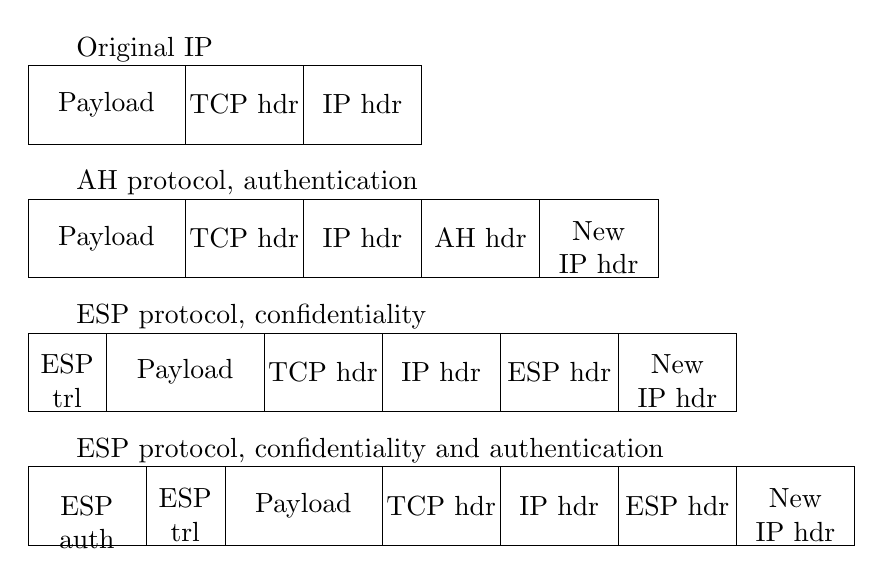
\begin{tikzpicture}
\pgftransformxscale{1.000000}
\pgftransformyscale{-1.000000}
\definecolor{dialinecolor}{rgb}{0.000000, 0.000000, 0.000000}
\pgfsetstrokecolor{dialinecolor}
\definecolor{dialinecolor}{rgb}{1.000000, 1.000000, 1.000000}
\pgfsetfillcolor{dialinecolor}
\pgfsetlinewidth{0.050000\du}
\pgfsetdash{}{0pt}
\pgfsetdash{}{0pt}
\pgfsetmiterjoin
\definecolor{dialinecolor}{rgb}{1.000000, 1.000000, 1.000000}
\pgfsetfillcolor{dialinecolor}
\fill (13.000000\du,10.100000\du)--(13.000000\du,11.100000\du)--(14.500000\du,11.100000\du)--(14.500000\du,10.100000\du)--cycle;
\definecolor{dialinecolor}{rgb}{0.000000, 0.000000, 0.000000}
\pgfsetstrokecolor{dialinecolor}
\draw (13.000000\du,10.100000\du)--(13.000000\du,11.100000\du)--(14.500000\du,11.100000\du)--(14.500000\du,10.100000\du)--cycle;
\pgfsetlinewidth{0.050000\du}
\pgfsetdash{}{0pt}
\pgfsetdash{}{0pt}
\pgfsetmiterjoin
\definecolor{dialinecolor}{rgb}{1.000000, 1.000000, 1.000000}
\pgfsetfillcolor{dialinecolor}
\fill (11.500000\du,8.400000\du)--(11.500000\du,9.400000\du)--(13.000000\du,9.400000\du)--(13.000000\du,8.400000\du)--cycle;
\definecolor{dialinecolor}{rgb}{0.000000, 0.000000, 0.000000}
\pgfsetstrokecolor{dialinecolor}
\draw (11.500000\du,8.400000\du)--(11.500000\du,9.400000\du)--(13.000000\du,9.400000\du)--(13.000000\du,8.400000\du)--cycle;
\pgfsetlinewidth{0.050000\du}
\pgfsetdash{}{0pt}
\pgfsetdash{}{0pt}
\pgfsetmiterjoin
\definecolor{dialinecolor}{rgb}{1.000000, 1.000000, 1.000000}
\pgfsetfillcolor{dialinecolor}
\fill (10.500000\du,6.700000\du)--(10.500000\du,7.700000\du)--(12.000000\du,7.700000\du)--(12.000000\du,6.700000\du)--cycle;
\definecolor{dialinecolor}{rgb}{0.000000, 0.000000, 0.000000}
\pgfsetstrokecolor{dialinecolor}
\draw (10.500000\du,6.700000\du)--(10.500000\du,7.700000\du)--(12.000000\du,7.700000\du)--(12.000000\du,6.700000\du)--cycle;
\pgfsetlinewidth{0.050000\du}
\pgfsetdash{}{0pt}
\pgfsetdash{}{0pt}
\pgfsetmiterjoin
\definecolor{dialinecolor}{rgb}{1.000000, 1.000000, 1.000000}
\pgfsetfillcolor{dialinecolor}
\fill (10.500000\du,5.000000\du)--(10.500000\du,6.000000\du)--(12.000000\du,6.000000\du)--(12.000000\du,5.000000\du)--cycle;
\definecolor{dialinecolor}{rgb}{0.000000, 0.000000, 0.000000}
\pgfsetstrokecolor{dialinecolor}
\draw (10.500000\du,5.000000\du)--(10.500000\du,6.000000\du)--(12.000000\du,6.000000\du)--(12.000000\du,5.000000\du)--cycle;
\pgfsetlinewidth{0.050000\du}
\pgfsetdash{}{0pt}
\pgfsetdash{}{0pt}
\pgfsetmiterjoin
\definecolor{dialinecolor}{rgb}{1.000000, 1.000000, 1.000000}
\pgfsetfillcolor{dialinecolor}
\fill (7.000000\du,5.000000\du)--(7.000000\du,6.000000\du)--(9.000000\du,6.000000\du)--(9.000000\du,5.000000\du)--cycle;
\definecolor{dialinecolor}{rgb}{0.000000, 0.000000, 0.000000}
\pgfsetstrokecolor{dialinecolor}
\draw (7.000000\du,5.000000\du)--(7.000000\du,6.000000\du)--(9.000000\du,6.000000\du)--(9.000000\du,5.000000\du)--cycle;
% setfont left to latex
\definecolor{dialinecolor}{rgb}{0.000000, 0.000000, 0.000000}
\pgfsetstrokecolor{dialinecolor}
\node at (8.000000\du,5.500000\du){Payload};
\pgfsetlinewidth{0.050000\du}
\pgfsetdash{}{0pt}
\pgfsetdash{}{0pt}
\pgfsetmiterjoin
\definecolor{dialinecolor}{rgb}{1.000000, 1.000000, 1.000000}
\pgfsetfillcolor{dialinecolor}
\fill (9.000000\du,5.000000\du)--(9.000000\du,6.000000\du)--(10.500000\du,6.000000\du)--(10.500000\du,5.000000\du)--cycle;
\definecolor{dialinecolor}{rgb}{0.000000, 0.000000, 0.000000}
\pgfsetstrokecolor{dialinecolor}
\draw (9.000000\du,5.000000\du)--(9.000000\du,6.000000\du)--(10.500000\du,6.000000\du)--(10.500000\du,5.000000\du)--cycle;
% setfont left to latex
\definecolor{dialinecolor}{rgb}{0.000000, 0.000000, 0.000000}
\pgfsetstrokecolor{dialinecolor}
\node at (11.250000\du,5.500000\du){IP hdr};
% setfont left to latex
\definecolor{dialinecolor}{rgb}{0.000000, 0.000000, 0.000000}
\pgfsetstrokecolor{dialinecolor}
\node at (9.750000\du,5.500000\du){TCP hdr};
\pgfsetlinewidth{0.050000\du}
\pgfsetdash{}{0pt}
\pgfsetdash{}{0pt}
\pgfsetmiterjoin
\definecolor{dialinecolor}{rgb}{1.000000, 1.000000, 1.000000}
\pgfsetfillcolor{dialinecolor}
\fill (7.000000\du,6.700000\du)--(7.000000\du,7.700000\du)--(9.000000\du,7.700000\du)--(9.000000\du,6.700000\du)--cycle;
\definecolor{dialinecolor}{rgb}{0.000000, 0.000000, 0.000000}
\pgfsetstrokecolor{dialinecolor}
\draw (7.000000\du,6.700000\du)--(7.000000\du,7.700000\du)--(9.000000\du,7.700000\du)--(9.000000\du,6.700000\du)--cycle;
% setfont left to latex
\definecolor{dialinecolor}{rgb}{0.000000, 0.000000, 0.000000}
\pgfsetstrokecolor{dialinecolor}
\node at (8.000000\du,7.200000\du){Payload};
\pgfsetlinewidth{0.050000\du}
\pgfsetdash{}{0pt}
\pgfsetdash{}{0pt}
\pgfsetmiterjoin
\definecolor{dialinecolor}{rgb}{1.000000, 1.000000, 1.000000}
\pgfsetfillcolor{dialinecolor}
\fill (9.000000\du,6.700000\du)--(9.000000\du,7.700000\du)--(10.500000\du,7.700000\du)--(10.500000\du,6.700000\du)--cycle;
\definecolor{dialinecolor}{rgb}{0.000000, 0.000000, 0.000000}
\pgfsetstrokecolor{dialinecolor}
\draw (9.000000\du,6.700000\du)--(9.000000\du,7.700000\du)--(10.500000\du,7.700000\du)--(10.500000\du,6.700000\du)--cycle;
% setfont left to latex
\definecolor{dialinecolor}{rgb}{0.000000, 0.000000, 0.000000}
\pgfsetstrokecolor{dialinecolor}
\node at (11.250000\du,7.200000\du){IP hdr};
% setfont left to latex
\definecolor{dialinecolor}{rgb}{0.000000, 0.000000, 0.000000}
\pgfsetstrokecolor{dialinecolor}
\node at (9.750000\du,7.200000\du){TCP hdr};
\pgfsetlinewidth{0.050000\du}
\pgfsetdash{}{0pt}
\pgfsetdash{}{0pt}
\pgfsetmiterjoin
\definecolor{dialinecolor}{rgb}{1.000000, 1.000000, 1.000000}
\pgfsetfillcolor{dialinecolor}
\fill (12.000000\du,6.700000\du)--(12.000000\du,7.700000\du)--(13.500000\du,7.700000\du)--(13.500000\du,6.700000\du)--cycle;
\definecolor{dialinecolor}{rgb}{0.000000, 0.000000, 0.000000}
\pgfsetstrokecolor{dialinecolor}
\draw (12.000000\du,6.700000\du)--(12.000000\du,7.700000\du)--(13.500000\du,7.700000\du)--(13.500000\du,6.700000\du)--cycle;
% setfont left to latex
\definecolor{dialinecolor}{rgb}{0.000000, 0.000000, 0.000000}
\pgfsetstrokecolor{dialinecolor}
\node at (12.750000\du,7.200000\du){AH hdr};
% setfont left to latex
\definecolor{dialinecolor}{rgb}{0.000000, 0.000000, 0.000000}
\pgfsetstrokecolor{dialinecolor}
\node[anchor=west] at (7.500000\du,4.800000\du){Original IP};
% setfont left to latex
\definecolor{dialinecolor}{rgb}{0.000000, 0.000000, 0.000000}
\pgfsetstrokecolor{dialinecolor}
\node[anchor=west] at (7.500000\du,6.500000\du){AH protocol, authentication};
\pgfsetlinewidth{0.050000\du}
\pgfsetdash{}{0pt}
\pgfsetdash{}{0pt}
\pgfsetmiterjoin
\definecolor{dialinecolor}{rgb}{1.000000, 1.000000, 1.000000}
\pgfsetfillcolor{dialinecolor}
\fill (8.000000\du,8.400000\du)--(8.000000\du,9.400000\du)--(10.000000\du,9.400000\du)--(10.000000\du,8.400000\du)--cycle;
\definecolor{dialinecolor}{rgb}{0.000000, 0.000000, 0.000000}
\pgfsetstrokecolor{dialinecolor}
\draw (8.000000\du,8.400000\du)--(8.000000\du,9.400000\du)--(10.000000\du,9.400000\du)--(10.000000\du,8.400000\du)--cycle;
% setfont left to latex
\definecolor{dialinecolor}{rgb}{0.000000, 0.000000, 0.000000}
\pgfsetstrokecolor{dialinecolor}
\node at (9.000000\du,8.900000\du){Payload};
\pgfsetlinewidth{0.050000\du}
\pgfsetdash{}{0pt}
\pgfsetdash{}{0pt}
\pgfsetmiterjoin
\definecolor{dialinecolor}{rgb}{1.000000, 1.000000, 1.000000}
\pgfsetfillcolor{dialinecolor}
\fill (10.000000\du,8.400000\du)--(10.000000\du,9.400000\du)--(11.500000\du,9.400000\du)--(11.500000\du,8.400000\du)--cycle;
\definecolor{dialinecolor}{rgb}{0.000000, 0.000000, 0.000000}
\pgfsetstrokecolor{dialinecolor}
\draw (10.000000\du,8.400000\du)--(10.000000\du,9.400000\du)--(11.500000\du,9.400000\du)--(11.500000\du,8.400000\du)--cycle;
% setfont left to latex
\definecolor{dialinecolor}{rgb}{0.000000, 0.000000, 0.000000}
\pgfsetstrokecolor{dialinecolor}
\node at (12.250000\du,8.900000\du){IP hdr};
% setfont left to latex
\definecolor{dialinecolor}{rgb}{0.000000, 0.000000, 0.000000}
\pgfsetstrokecolor{dialinecolor}
\node at (10.750000\du,8.900000\du){TCP hdr};
\pgfsetlinewidth{0.050000\du}
\pgfsetdash{}{0pt}
\pgfsetdash{}{0pt}
\pgfsetmiterjoin
\definecolor{dialinecolor}{rgb}{1.000000, 1.000000, 1.000000}
\pgfsetfillcolor{dialinecolor}
\fill (13.000000\du,8.400000\du)--(13.000000\du,9.400000\du)--(14.500000\du,9.400000\du)--(14.500000\du,8.400000\du)--cycle;
\definecolor{dialinecolor}{rgb}{0.000000, 0.000000, 0.000000}
\pgfsetstrokecolor{dialinecolor}
\draw (13.000000\du,8.400000\du)--(13.000000\du,9.400000\du)--(14.500000\du,9.400000\du)--(14.500000\du,8.400000\du)--cycle;
% setfont left to latex
\definecolor{dialinecolor}{rgb}{0.000000, 0.000000, 0.000000}
\pgfsetstrokecolor{dialinecolor}
\node at (13.750000\du,8.900000\du){ESP hdr};
\pgfsetlinewidth{0.050000\du}
\pgfsetdash{}{0pt}
\pgfsetdash{}{0pt}
\pgfsetmiterjoin
\definecolor{dialinecolor}{rgb}{1.000000, 1.000000, 1.000000}
\pgfsetfillcolor{dialinecolor}
\fill (7.000000\du,8.400000\du)--(7.000000\du,9.400000\du)--(8.000000\du,9.400000\du)--(8.000000\du,8.400000\du)--cycle;
\definecolor{dialinecolor}{rgb}{0.000000, 0.000000, 0.000000}
\pgfsetstrokecolor{dialinecolor}
\draw (7.000000\du,8.400000\du)--(7.000000\du,9.400000\du)--(8.000000\du,9.400000\du)--(8.000000\du,8.400000\du)--cycle;
% setfont left to latex
\definecolor{dialinecolor}{rgb}{0.000000, 0.000000, 0.000000}
\pgfsetstrokecolor{dialinecolor}
\node at (7.500000\du,8.804583\du){ESP};
% setfont left to latex
\definecolor{dialinecolor}{rgb}{0.000000, 0.000000, 0.000000}
\pgfsetstrokecolor{dialinecolor}
\node at (7.500000\du,9.227917\du){trl};
% setfont left to latex
\definecolor{dialinecolor}{rgb}{0.000000, 0.000000, 0.000000}
\pgfsetstrokecolor{dialinecolor}
\node[anchor=west] at (7.500000\du,8.200000\du){ESP protocol, confidentiality};
\pgfsetlinewidth{0.050000\du}
\pgfsetdash{}{0pt}
\pgfsetdash{}{0pt}
\pgfsetmiterjoin
\definecolor{dialinecolor}{rgb}{1.000000, 1.000000, 1.000000}
\pgfsetfillcolor{dialinecolor}
\fill (9.500000\du,10.100000\du)--(9.500000\du,11.100000\du)--(11.500000\du,11.100000\du)--(11.500000\du,10.100000\du)--cycle;
\definecolor{dialinecolor}{rgb}{0.000000, 0.000000, 0.000000}
\pgfsetstrokecolor{dialinecolor}
\draw (9.500000\du,10.100000\du)--(9.500000\du,11.100000\du)--(11.500000\du,11.100000\du)--(11.500000\du,10.100000\du)--cycle;
% setfont left to latex
\definecolor{dialinecolor}{rgb}{0.000000, 0.000000, 0.000000}
\pgfsetstrokecolor{dialinecolor}
\node at (10.500000\du,10.600000\du){Payload};
\pgfsetlinewidth{0.050000\du}
\pgfsetdash{}{0pt}
\pgfsetdash{}{0pt}
\pgfsetmiterjoin
\definecolor{dialinecolor}{rgb}{1.000000, 1.000000, 1.000000}
\pgfsetfillcolor{dialinecolor}
\fill (11.500000\du,10.100000\du)--(11.500000\du,11.100000\du)--(13.000000\du,11.100000\du)--(13.000000\du,10.100000\du)--cycle;
\definecolor{dialinecolor}{rgb}{0.000000, 0.000000, 0.000000}
\pgfsetstrokecolor{dialinecolor}
\draw (11.500000\du,10.100000\du)--(11.500000\du,11.100000\du)--(13.000000\du,11.100000\du)--(13.000000\du,10.100000\du)--cycle;
% setfont left to latex
\definecolor{dialinecolor}{rgb}{0.000000, 0.000000, 0.000000}
\pgfsetstrokecolor{dialinecolor}
\node at (13.750000\du,10.600000\du){IP hdr};
% setfont left to latex
\definecolor{dialinecolor}{rgb}{0.000000, 0.000000, 0.000000}
\pgfsetstrokecolor{dialinecolor}
\node at (12.250000\du,10.600000\du){TCP hdr};
\pgfsetlinewidth{0.050000\du}
\pgfsetdash{}{0pt}
\pgfsetdash{}{0pt}
\pgfsetmiterjoin
\definecolor{dialinecolor}{rgb}{1.000000, 1.000000, 1.000000}
\pgfsetfillcolor{dialinecolor}
\fill (14.500000\du,10.100000\du)--(14.500000\du,11.100000\du)--(16.000000\du,11.100000\du)--(16.000000\du,10.100000\du)--cycle;
\definecolor{dialinecolor}{rgb}{0.000000, 0.000000, 0.000000}
\pgfsetstrokecolor{dialinecolor}
\draw (14.500000\du,10.100000\du)--(14.500000\du,11.100000\du)--(16.000000\du,11.100000\du)--(16.000000\du,10.100000\du)--cycle;
% setfont left to latex
\definecolor{dialinecolor}{rgb}{0.000000, 0.000000, 0.000000}
\pgfsetstrokecolor{dialinecolor}
\node at (15.250000\du,10.600000\du){ESP hdr};
\pgfsetlinewidth{0.050000\du}
\pgfsetdash{}{0pt}
\pgfsetdash{}{0pt}
\pgfsetmiterjoin
\definecolor{dialinecolor}{rgb}{1.000000, 1.000000, 1.000000}
\pgfsetfillcolor{dialinecolor}
\fill (8.500000\du,10.100000\du)--(8.500000\du,11.100000\du)--(9.500000\du,11.100000\du)--(9.500000\du,10.100000\du)--cycle;
\definecolor{dialinecolor}{rgb}{0.000000, 0.000000, 0.000000}
\pgfsetstrokecolor{dialinecolor}
\draw (8.500000\du,10.100000\du)--(8.500000\du,11.100000\du)--(9.500000\du,11.100000\du)--(9.500000\du,10.100000\du)--cycle;
% setfont left to latex
\definecolor{dialinecolor}{rgb}{0.000000, 0.000000, 0.000000}
\pgfsetstrokecolor{dialinecolor}
\node at (9.000000\du,10.504583\du){ESP};
% setfont left to latex
\definecolor{dialinecolor}{rgb}{0.000000, 0.000000, 0.000000}
\pgfsetstrokecolor{dialinecolor}
\node at (9.000000\du,10.927917\du){trl};
\pgfsetlinewidth{0.050000\du}
\pgfsetdash{}{0pt}
\pgfsetdash{}{0pt}
\pgfsetmiterjoin
\definecolor{dialinecolor}{rgb}{1.000000, 1.000000, 1.000000}
\pgfsetfillcolor{dialinecolor}
\fill (7.000000\du,10.100000\du)--(7.000000\du,11.100000\du)--(8.500000\du,11.100000\du)--(8.500000\du,10.100000\du)--cycle;
\definecolor{dialinecolor}{rgb}{0.000000, 0.000000, 0.000000}
\pgfsetstrokecolor{dialinecolor}
\draw (7.000000\du,10.100000\du)--(7.000000\du,11.100000\du)--(8.500000\du,11.100000\du)--(8.500000\du,10.100000\du)--cycle;
% setfont left to latex
\definecolor{dialinecolor}{rgb}{0.000000, 0.000000, 0.000000}
\pgfsetstrokecolor{dialinecolor}
\node at (7.750000\du,10.600000\du){ESP};
% setfont left to latex
\definecolor{dialinecolor}{rgb}{0.000000, 0.000000, 0.000000}
\pgfsetstrokecolor{dialinecolor}
\node at (7.750000\du,11.023333\du){auth};
% setfont left to latex
\definecolor{dialinecolor}{rgb}{0.000000, 0.000000, 0.000000}
\pgfsetstrokecolor{dialinecolor}
\node[anchor=west] at (7.500000\du,9.900000\du){ESP protocol, confidentiality and authentication};
\pgfsetlinewidth{0.050000\du}
\pgfsetdash{}{0pt}
\pgfsetdash{}{0pt}
\pgfsetmiterjoin
\definecolor{dialinecolor}{rgb}{1.000000, 1.000000, 1.000000}
\pgfsetfillcolor{dialinecolor}
\fill (13.500000\du,6.700000\du)--(13.500000\du,7.700000\du)--(15.000000\du,7.700000\du)--(15.000000\du,6.700000\du)--cycle;
\definecolor{dialinecolor}{rgb}{0.000000, 0.000000, 0.000000}
\pgfsetstrokecolor{dialinecolor}
\draw (13.500000\du,6.700000\du)--(13.500000\du,7.700000\du)--(15.000000\du,7.700000\du)--(15.000000\du,6.700000\du)--cycle;
% setfont left to latex
\definecolor{dialinecolor}{rgb}{0.000000, 0.000000, 0.000000}
\pgfsetstrokecolor{dialinecolor}
\node at (14.250000\du,7.104583\du){New};
% setfont left to latex
\definecolor{dialinecolor}{rgb}{0.000000, 0.000000, 0.000000}
\pgfsetstrokecolor{dialinecolor}
\node at (14.250000\du,7.527917\du){IP hdr};
\pgfsetlinewidth{0.050000\du}
\pgfsetdash{}{0pt}
\pgfsetdash{}{0pt}
\pgfsetmiterjoin
\definecolor{dialinecolor}{rgb}{1.000000, 1.000000, 1.000000}
\pgfsetfillcolor{dialinecolor}
\fill (14.500000\du,8.400000\du)--(14.500000\du,9.400000\du)--(16.000000\du,9.400000\du)--(16.000000\du,8.400000\du)--cycle;
\definecolor{dialinecolor}{rgb}{0.000000, 0.000000, 0.000000}
\pgfsetstrokecolor{dialinecolor}
\draw (14.500000\du,8.400000\du)--(14.500000\du,9.400000\du)--(16.000000\du,9.400000\du)--(16.000000\du,8.400000\du)--cycle;
% setfont left to latex
\definecolor{dialinecolor}{rgb}{0.000000, 0.000000, 0.000000}
\pgfsetstrokecolor{dialinecolor}
\node at (15.250000\du,8.804583\du){New};
% setfont left to latex
\definecolor{dialinecolor}{rgb}{0.000000, 0.000000, 0.000000}
\pgfsetstrokecolor{dialinecolor}
\node at (15.250000\du,9.227917\du){IP hdr};
\pgfsetlinewidth{0.050000\du}
\pgfsetdash{}{0pt}
\pgfsetdash{}{0pt}
\pgfsetmiterjoin
\definecolor{dialinecolor}{rgb}{1.000000, 1.000000, 1.000000}
\pgfsetfillcolor{dialinecolor}
\fill (16.000000\du,10.100000\du)--(16.000000\du,11.100000\du)--(17.500000\du,11.100000\du)--(17.500000\du,10.100000\du)--cycle;
\definecolor{dialinecolor}{rgb}{0.000000, 0.000000, 0.000000}
\pgfsetstrokecolor{dialinecolor}
\draw (16.000000\du,10.100000\du)--(16.000000\du,11.100000\du)--(17.500000\du,11.100000\du)--(17.500000\du,10.100000\du)--cycle;
% setfont left to latex
\definecolor{dialinecolor}{rgb}{0.000000, 0.000000, 0.000000}
\pgfsetstrokecolor{dialinecolor}
\node at (16.750000\du,10.504583\du){New};
% setfont left to latex
\definecolor{dialinecolor}{rgb}{0.000000, 0.000000, 0.000000}
\pgfsetstrokecolor{dialinecolor}
\node at (16.750000\du,10.927917\du){IP hdr};
\end{tikzpicture}

	}
}
\caption{IPsec (a) transport and (b) tunnel overheads}{Tunnel mode adds a custom IP header and moves the AH/ESP header in front of the original IP header. Note: ``trl" stands for ``trailer", ``hdr" for ``header", reproduced from~\cite{Xenakis20063225}}
\label{fig:ipsec-transport-tunnel}
\end{figure}

RFC 7321~\cite{rfc7321} defines the support for only three AES modes: CBC, CTR and GCM.





%%%%%%%%%%%%%%%%%%
% We can not invoke a verbatim environement from an other command. We thus save is inside a box and we will invoke said box later.
\newsavebox\myv

\begin{lrbox}{\myv}\begin{minipage}{\textwidth}
\begin{verbatim}
0                   1                   2                   3
 0 1 2 3 4 5 6 7 8 9 0 1 2 3 4 5 6 7 8 9 0 1 2 3 4 5 6 7 8 9 0 1
+-+-+-+-+-+-+-+-+-+-+-+-+-+-+-+-+-+-+-+-+-+-+-+-+-+-+-+-+-+-+-+-+ -----------
|               Security Parameters Index (SPI)                 |      ^Int.
+-+-+-+-+-+-+-+-+-+-+-+-+-+-+-+-+-+-+-+-+-+-+-+-+-+-+-+-+-+-+-+-+      |Cov-
|                      Sequence Number                          |      |ered
+-+-+-+-+-+-+-+-+-+-+-+-+-+-+-+-+-+-+-+-+-+-+-+-+-+-+-+-+-+-+-+-+---   | ----
|                    IV (optional)                              | ^ p  |   ^
+-+-+-+-+-+-+-+-+-+-+-+-+-+-+-+-+-+-+-+-+-+-+-+-+-+-+-+-+-+-+-+-+ | a  |   |
|                    Rest of Payload Data  (variable)           | | y  |Conf.
~                                                               ~ | l  |Cov-
|                                                               | | o  |ered*
+               +-+-+-+-+-+-+-+-+-+-+-+-+-+-+-+-+-+-+-+-+-+-+-+-+ | a  |   |
|               |         TFC Padding * (optional, variable)    | v d  |   |
+-+-+-+-+-+-+-+-+         +-+-+-+-+-+-+-+-+-+-+-+-+-+-+-+-+-+-+-+---   |   |
|                         |        Padding (0-255 bytes)        |      |   |
+-+-+-+-+-+-+-+-+-+-+-+-+-+     +-+-+-+-+-+-+-+-+-+-+-+-+-+-+-+-+      |   |
|                               |  Pad Length   | Next Header   |      v   v
+-+-+-+-+-+-+-+-+-+-+-+-+-+-+-+-+-+-+-+-+-+-+-+-+-+-+-+-+-+-+-+-+------------
|         Integrity Check Value-ICV   (variable)                |
~                                                               ~
|                                                               |
+-+-+-+-+-+-+-+-+-+-+-+-+-+-+-+-+-+-+-+-+-+-+-+-+-+-+-+-+-+-+-+-+
\end{verbatim}
\end{minipage}\end{lrbox}

\begin{figure}
\center
	\resizebox{.8\linewidth}{!}{%
	\usebox\myv
	}
\caption{ESP packet structure}{as defined in RFC 4303~\cite{rfc4303}.}
\label{fig:esp-packet-structure}
\end{figure}